\documentclass{article}

\PassOptionsToPackage{numbers,compress}{natbib}
\usepackage[final,preprint]{nips2023}

\usepackage[utf8]{inputenc}
\usepackage[T1]{fontenc}
\usepackage{times}
\usepackage{amsmath, amsfonts, amssymb}
\usepackage{graphicx}
\usepackage{booktabs}
\usepackage{caption}
\usepackage{tikz}
\usetikzlibrary{arrows.meta,positioning,fit,calc,shapes.geometric}
\usepackage{algpseudocode}
\usepackage{algorithm}
\usepackage{setspace}
\usepackage{comment}
\usepackage{amsthm}
\usepackage{subcaption}
\usepackage{hyperref}
\usepackage{url}
\usepackage{latexsym}
\usepackage{abstract}
\usepackage{float}
\title{A Confidence-Based Watermark for Diffusion Language Models}
\makeatletter
\let\@notice\relax
\makeatother

\author{
Elijah Feldman \\
TJHSST \\
Annandale, USA \\
2028efeldman@tjhsst.edu
\and
Samuel Zhang \\
TJHSST \\
Annandale, USA \\
2028szhang@tjhsst.edu
}
\date{}

\newtheorem{theorem}{Theorem}[section]
\newtheorem{proposition}[theorem]{Proposition}
\renewcommand{\qedsymbol}{\ensuremath{\blacksquare}}

\renewcommand{\abstractname}{ABSTRACT}
\renewcommand{\abstractnamefont}{\large\normalfont}
\renewcommand{\abstracttextfont}{\normalfont}

\setlength{\absleftindent}{0pt}
\setlength{\absrightindent}{0pt}
\setlength{\abstitleskip}{0.6em}
\begin{document}
\maketitle
\pagestyle{empty}
\nocite{*}

\begin{abstract}
\begingroup
\setstretch{1.08}
\fontsize{11}{13}\selectfont
We introduce a joint token-and-order watermark for diffusion language models (DLMs),
a class of large language models that generate tokens in a non-autoregressive, arbitrary order.
Due to their architecture, DLMs offer advantages over traditional autoregressive language models (ARLMs),
being able to iterate on a solution faster and correct errors during the generation process. Most existing
watermarking methods for ARLMs rely on access to previously generated tokens, making them incompatible with DLMs.
At each generation step, a DLM decides token predictions to replace masked indices, and which positions to actually unmask, the latter
of which is chosen by a confidence metric. Existing DLM watermarking approaches only modify either the token distribution
or the unmasking order. Our joint token-and-order DLM watermark alters both to maximize the expected number of green tokens under a
certain KL per token threshold during generation. On LLaDA-8B with prompts from WaterBench, with matched KL per token, our joint watermark
raises the true positive rate at $<10^{-4}$ from 0.75 to 0.90 over the token-only watermark of Gloaguen et al., and outperforms the order-only dgMARK.


\endgroup




\end{abstract}

\section{Introduction}


Traditional autoregressive language models (ARLMs) have shown remarkable performance (\cite{llama3herd2024}).
Diffusion language models (DLMs) have arisen as a new class of transformers. Instead of generating the output one
token at a time, from left to right, DLMs perform similar to their image generation counterparts, starting with noise
 and refining its predictions in parallel. Several new DLMs have reached similar performance at faster response times
  (\cite{nie2025large, google2025gemini, ye2025dream7b}. They also have built in error correction, as well as
  bidirectional context, which can enable more coherent outputs. Previous works have proposed ARLM watermarks,
  which bias the probability distribution of the model's predictions. The result is a signal imperceptible to humans
   but can be traced. ARLM watermarks have already been adopted in consumer models, and are advocated for with
   regulation. However, the unique architecture of DLMs has led to the development of two kinds of watermarking methods adapted for them.
   One scheme uses context hashing in expectation to pseudorandomly modify the token logit distribution \cite{gloaguen2025dlm}. The other method
   uses a keyed rule to reorder which positions are unmasked during diffusion generation \cite{hong2026dgmark}. We unify these two techniques and
   contribute a joint watermark that perturbs both token predictions at indices and the confidence metric used to select unmasking order, adding a signal
   inperceptible to the human eye but detectable with a specific key.


\textbf{Diffusion Language Models}
DLMs begin with a fixed length unknown output sequence, denoted by a set of [MASK] tokens. At each generation step, the model provides a probability distribution for its prediction for each token, and assigns a confidence score to each of its predictions. The model will unmask its predictions, and then remask the tokens with the lowest confidence scores. The model will continue this until all tokens are unmasked, producing a coherent output.


\textbf{ARLM watermarks}
Existing watermarks for ARLMs use a green-red token split. This green and red list is chosen before each word is generated, and the model's predictions are biased towards green list tokens. These watermarks often use the hash of the previous token to seed the random number generator that decides on the red-green split. This hash can not be used, since DLM generation does not always have the previous token generated.


\textbf{Existing DLM watermarks}
Gloaguen et al. \cite{gloaguen2025dlm} adapt the green-red list to diffusion models by computing the context hashes in expectation over masked tokens and applying a logit bias based on these expected hashes.
dgMARK \cite{hong2026dgmark} leaves token probabilities unchanged and instead prioritizes unmasking indices whose token prediction satisfies a keyed parity-based rule. Current methods watermark either on token distribution or unmasking order, not both.


\textbf{This work: A Joint Token-and-Order Watermark for Diffusion Language Models}
In this work, the DLM watermark is split into a token component and an order component at each diffusion generation step.
The token component alters the logit distribution at each position, and the order component modifies the confidence scores the model uses to
select which positions to unmask. We maximize the expected number of green tokens in the final output text under a specified KL per token
threshold, adding a separate bias to each component to accomplish this. The token bias is added to the logits and modeled after the energy-based bias of
Gloaguen et al. The order bias is added to each position's confidence score and equals the expected gain in green tokens
from unmasking a certain position at this particular diffusion generation step rather than at a later one. Setting either bias strength to zero effectively makes
the joint watermark a single-component one. Like ARLM watermarks, our detection algorithm counts the
number of green tokens in a section of text and performs a binomial test for significance.


\textbf{Main Contributions} Our main contributions are:
\begin{itemize}
   \item We establish a joint token-and-order watermark that applies bias to both the token distribution and the unmasking order of a DLM under a per-token KL-constrained objective, with token-only and order-only watermarks as special cases.
   \item We introduce an order component score, which measures the expected green-token gain from unmasking a position at the current generation step rather than a later one; this lets the token bias act on fixed context.
   \item We compare our joint watermark against both Gloaguen et al. and dgMARK algorithms on LLaDA-8B under the same benchmarks, green list and detector, and show higher detection at matched token-level KL.
\end{itemize}



\section{Background}
\textbf{Auto-Regressive Language Models (ARLMs)} Large language models \cite{devlin2019bertpretrainingdeepbidirectional} are
    given a vocabulary of $\sum$ and text sequences \(\omega = (w_1,\dots,w_T) \in \Sigma^T\). In an auto-regressive model, $\theta$
    denotes the parameters that define a conditional probability distribution over the next token given its predecessors,
  $p_\theta(w_t
    | w_{1:t-1})$. The training objective is to choose \(\theta\) so that \(p_\theta\) approximates the data distribution
    \(p_{\text{data}}\) by minimizing the expected negative log-likelihood.

  \textbf{Diffusion Language Models (DLMs)} For diffusion language models, the goal is to learn the conditional
  distributions that will invert a corruption process. The model aims to transform a masked, noisy output sequence to samples from \(p_{\text{data}}\). The goal is to minimize a cross entropy loss only on the masked tokens. At each refinement step, the model unmasks its most confident predictions while re-masking the tokens with the lowest confidence for subsequent processing. These models have been implemented in several prominent systems, such as LLaDA, and similar diffusion-based approaches have been explored in models like Gemini Diffusion.
  \newline
  \textbf{LLM Watermark}
  A watermark is a hidden statistical signal embedded in machine-generated text to determine if it is AI generated. A watermark changes the model’s word choices during generation, guiding it towards a particular pattern that would be unlikely to appear randomly. Changes made by the watermark are designed to be imperceptible to a human reader, preserving text quality and coherence. However, a
  detection algorithm with access to a secret key can analyze the text and detect a pattern, verifying that the text was generated by a
  watermarked model.

   A language model watermark can be formally defined as a set of three components: an embedding process \(E\), a sampling procedure
  \(G\), and a
    detection function \(D\). These components operate on the underlying token distributions of a given language model.

    Let \(p_\theta(w_t | c)\) be the original conditional probability distribution over the vocabulary \(\Sigma\) that the language
  model \(\theta\)
    assigns to the token \(w_t\) given a relevant context \(c\).

      1. Embedding Process (\(E\)): The embedding process transforms the original distribution \(p_\theta\) into a watermarked
         distribution \(p'_\theta\).
        This transformation is conditioned on a message or secret key \(k\).
        \[ E(p_\theta(w_t | c), k) \rightarrow p'_\theta(w_t | c, k) \]
        To preserve the quality of the generated text, the watermarked distribution must remain close to the original. This is
  formally constrained by
    requiring that a statistical distance, such as the Kullback-Leibler (KL) divergence, between the two distributions is bounded by a
  small value
    \(\epsilon\):
        \[ D_{KL}(p'_\theta || p_\theta) \leq \epsilon \]

      2. Sampling Procedure (\(G\)): The generation or sampling procedure produces a watermarked text \(\omega = (w_1, \dots, w_T)\)
         by drawing tokens
        from the watermarked distribution \(p'_\theta\). For autoregressive models, this involves sequential sampling: \(w_t \sim
  p'_\theta(w_t |
        w_{1:t-1}, k)\). For Diffusion Language Models (DLMs), this involves an iterative refinement process where the model
  repeatedly samples and
        updates tokens across the sequence, guided by \(p'_\theta\) to invert a corruption process. In both cases, the context \(c\)
  in \(p'_\theta(w_t |
        c, k)\) represents the relevant information at each decision point.

      3. Detection Function (\(D\)): The detection function determines if a given text \(\omega\) contains the watermark. This is a
         hypothesis testing
        problem with two hypotheses:
          Null Hypothesis (\(H_0\)): The text was generated by the original model, \(\omega \sim p_\theta\).
          Alternative Hypothesis (\(H_1\)): The text was generated by the watermarked model, \(\omega \sim p'_\theta\).

        The detector computes a test statistic \(S(\omega, k)\) and compares it to a threshold \(\tau\). The text is classified as
  watermarked if
    \(S(\omega, k) > \tau\). The choice of \(\tau\) determines the trade-off between the False Positive Rate (Type I error,
  \(\alpha\)) and the True
    Positive Rate (power, \(1-\beta\)).

  \textbf{Properties of an Effective Watermark}
  An effective watermarking scheme is expected to have several key properties:
  \begin{itemize}
      \item \textbf{Text Quality Preservation} The watermark should not clearly degrade the quality, fluency, or correctness of
  generated text. The KL-divergence constraint on \(p'_\theta\) is a formal measure of this.
      \item \textbf{Robustness:} The statistical signal must be robust to common text alterations. A user attempting to remove the
  watermark might paraphrase sentences, insert or delete words, or use another model to revise the text. The detection function \(D\)
  should still identify the watermark with after such modifications.
      \item \textbf{Security:} It should be computationally infeasible to detect the watermark, forge it in human-written
  text, or remove it from generated text without access to the secret key \(k\).
      \item \textbf{Reliability:} The watermark must be reliably detectable, achieving a high True Positive Rate while maintaining a low False Positive Rate to avoid falsely accusing human authors.
  \end{itemize}

  \textbf{Prior Work in LLM Watermarking}
  The most prominent watermarking scheme for ARLMs \cite{kirchenbauer2023} partitions the vocabulary into a "green list" and a "red list" at each time step. The partition is determined pseudorandomly using a secret key and the hash of the preceding token sequence. The embedding process \(E\) slightly increases the probabilities of tokens on the green list before sampling. The detection function \(D\) involves counting the number of green-listed tokens in a given text to determine whether it statistically significant. While effective, this reliance on a fixed context window makes it incompatible with the non-sequential generation of DLMs. Early work in watermarking DLMs[citation idk how to do pls help] has attempted to adapt this method by computing context hashes in expectation over the masked tokens.
\section{Approach}
\textbf{Overview.} Our watermark leverages the unique properties of DLMs: (1) parallel token generation allows us to define pairwise relationships between tokens, and (2) confidence-based remasking provides a natural biasing mechanism. Unlike autoregressive watermarks that bias token probabilities directly, we bias confidence scores in logit space, which determines the order in which tokens are unmasked during the diffusion process.
\subsection*{Design Rationale}

\textbf{Optimization Problem}

Let $\mathbf{p} \in (0,1)^N$ denote the original token confidences predicted by the Diffusion Language Model (DLM) for a sequence of length $N$, where $p_i$ is the probability of keeping token $i$. Let $\mathbf{\hat{p}} \in (0,1)^N$ denote the modified (watermarked) token confidences. 

We define the expected green-list pair count for token $i$ as $g_i \in \mathbb{R}_{\geq 0}$. The gain in the expected satisfaction rate is directly proportional to the shift in probability $\Delta p_i = \hat{p}_i - p_i$. We frame the watermarking process as an optimization problem where we seek to maximize the expected satisfaction rate subject to a maximum allowable distortion budget $\epsilon$, measured by the Kullback-Leibler (KL) divergence between the modified and original Bernoulli distributions:

\begin{equation}
\begin{aligned}
& \max_{\mathbf{\hat{p}}} \quad \sum_{i=1}^{N} (\hat{p}_i - p_i) g_i \\
& \text{subject to} \quad \sum_{i=1}^{N} D_{\text{KL}}\big(\text{Bern}(\hat{p}_i) \parallel \text{Bern}(p_i)\big) \leq \epsilon
\end{aligned}
\end{equation}

To relate the probability shift $\Delta p_i$ to the applied logit bias $b_i$, recall that the modified probability is computed in the log-odds (logit) space:
\begin{equation}
\hat{p}_i = \sigma\big(\sigma^{-1}(p_i) + b_i\big)
\end{equation}
where $\sigma(\cdot)$ is the sigmoid function. For small bias $b_i$, the first-order Taylor expansion gives the transfer function mapping bias to probability shift:
\begin{equation}
\Delta p_i \approx b_i \cdot p_i(1 - p_i)
\end{equation}

Furthermore, for small $\Delta p_i$, the KL divergence can be approximated using the Fisher Information $I(p_i) = \frac{1}{p_i(1-p_i)}$:
\begin{equation}
D_{\text{KL}}\big(\text{Bern}(\hat{p}_i) \parallel \text{Bern}(p_i)\big) \approx \frac{1}{2} (\Delta p_i)^2 I(p_i) = \frac{1}{2} \frac{(\Delta p_i)^2}{p_i(1-p_i)} \approx \frac{1}{2} b_i^2 \cdot p_i(1-p_i)
\end{equation}

Substituting these approximations into our optimization problem, we define the Lagrangian $\mathcal{L}(\mathbf{b}, \lambda)$ with respect to the logit bias vector $\mathbf{b}$ and a Lagrange multiplier $\lambda \geq 0$:
\begin{equation}
\mathcal{L}(\mathbf{b}, \lambda) = \sum_{i=1}^{N} \Big( b_i \cdot p_i(1-p_i) \cdot g_i \Big) - \lambda \left( \sum_{i=1}^{N} \frac{1}{2} b_i^2 \cdot p_i(1-p_i) - \epsilon \right)
\end{equation}

\textbf{energy formulation}

Let $p_i$ be the original token confidence, $\hat{p}_i = \sigma(L_i + b_i)$ be the modified probability after applying bias $b_i$, $g_i$ be the expected green-list count (the satisfaction gradient), and $\delta$ be the KL-divergence scaling factor. We define the total energy function $\mathcal{E}(b_i)$ as the combination of the predictive distortion (KL divergence), the $L_2$ bias penalty parameterized by $\lambda_{\text{l2}}$, and the negative expected satisfaction rate:

\begin{equation}
\mathcal{E}(b_i) = \frac{1}{\delta} D_{\text{KL}}\big(\text{Bern}(\hat{p}_i) \parallel \text{Bern}(p_i)\big) + \lambda_{\text{l2}} b_i^2 - g_i \hat{p}_i
\end{equation}

To find the state of lowest energy, we compute the exact derivative of $\mathcal{E}$ with respect to the bias $b_i$. Using the Fisher Information approximation for small shifts, the derivative of the KL divergence with respect to the logit bias is $b_i \hat{p}_i(1-\hat{p}_i)$. Furthermore, the derivative of the sigmoid probability $\hat{p}_i$ with respect to its logit is the variance $\hat{p}_i(1-\hat{p}_i)$. Setting the gradient to zero yields:

\begin{equation}
\frac{\partial \mathcal{E}}{\partial b_i} = \frac{1}{\delta} b_i \hat{p}_i(1-\hat{p}_i) + 2\lambda_{\text{l2}} b_i - g_i \hat{p}_i(1-\hat{p}_i) = 0
\end{equation}

Rearranging this to solve for the optimal bias $b_i^*$ yields the following stationary point:

\begin{equation}
b_i^* = \frac{g_i \hat{p}_i(1-\hat{p}_i)}{\frac{1}{\delta} \hat{p}_i(1-\hat{p}_i) + 2\lambda_{\text{l2}}}
\end{equation}


\textbf{Pairwise rules vs. individual tokens.} Unlike prior work that classifies individual tokens as green/red, we define green/red pairs. This reduces the number of biased positions (fewer modifications to the generation process) while maintaining detection strength.

\textbf{Context window $C = \{-2, -1, 1, 2\}$.} We use a symmetric window excluding position 0 (self) to capture local token dependencies while keeping computational cost manageable. Larger windows increase detection strength but slow generation.

\textbf{Confidence weighting.} For masked neighbors, we weight by their confidence $c_{i+j}$ rather than uniformly. This accounts for uncertainty: a green pair with a high-confidence neighbor provides stronger signal than one with low confidence.

\textbf{Logit-space biasing.} Directly adding $\delta \cdot \sigma_i$ to probabilities $c_i \in (0,1)$ would produce invalid values. We transform to logit space via inverse sigmoid, apply the bias, then transform back via sigmoid: $c'_i = \sigma(\sigma^{-1}(c_i) + \delta \cdot \sigma_i)$.
\subsection{Pair Rule}
Let $C = \{-2, -1, 1, 2\}$ denote the relative indices of the local neighborhood for the current position $k$. Let $v \in \Sigma$ be a candidate token at position $k$, and let $\hat{u}_{k+j}$ represent the estimated token at neighbor position $k+j$ (using the ground truth token if unmasked, or the model's current hard prediction $x_0$ if masked).

First, we define a base hash function $h(a, b)$ that operates on a sorted pair of tokens:
\begin{equation}
    h(a, b) = \text{LSB}\left(\text{SHA256}\bigl(K \parallel \min(a, b) \parallel \text{"|"} \parallel \max(a, b)\bigr)\right) \in \{0, 1\}
\end{equation}
where $K$ is a secret key and $\text{LSB}$ denotes the least significant bit.

To enforce anti-symmetry and discourage repetition, we define the directed validity function $\phi(a, b)$. This function returns 1 if the ordered sequence $a \rightarrow b$ is valid ("green"), and 0 otherwise:
\begin{equation}
    \phi(a, b) = 
    \begin{cases} 
        h(a, b) & \text{if } a \le b \\
        1 - h(a, b) & \text{if } a > b 
    \end{cases}
\end{equation}
Under this rule, if the transition $a \rightarrow b$ is green, the reverse transition $b \rightarrow a$ is necessarily red.
\subsection{Our Watermark}
\noindent
\begin{minipage}[t]{0.38\textwidth}
\vspace{0pt}
\small
\raggedright
During generation, we define our watermark with (Algorithm 1). Specifically, we start by converting confidence scores from probabilities $\in$ (0,1) to logits through an inverse sigmoid. At each diffusion step $i$, we loop over each masked token position and compute a local support score $\sigma_i$ from nearby tokens in the context window (weighted by confidence when a neighbor is still masked). We then bias confidence logits by $\delta \cdot \sigma_i$.

This bias affects which positions are revealed earlier: the DLM remasking procedure unmasks all tokens, then re-masks the lowest-confidence tokens, and repeats until all tokens remain unmasked.

For detection, we iterate over each position and calculate the proportion of green pairs. We then apply a binomial test to test for a significant number of green pairs.

\end{minipage}
\begin{minipage}[t]{0.6\textwidth}
\vspace{0pt}
\vspace{-3mm}
\begin{algorithm}[H]
\caption{Watermark Generation}
\begin{algorithmic}[1]
\Require Proposed seq $x \in V^L$, Fixed seq $T \in V^L$, Mask $m \in \{0,1\}^L$, Conf $c \in (0,1)^L$, Key $k$, Context window $C$, Strength $\delta$, Hash $f_k$.
\Ensure Modified confidence $c'$.

\State $\ell \gets \ln(c \oslash (1 - c))$ \Comment{Convert confidence to logits}
\State $c' \gets \text{set } c_i = -\infty \text{ for all } i \text{ where } m_i = 0$
\For{each masked index $i \in \{i \mid m_i = 1\}$}
    \State $\sigma_i \gets \sum_{j \in C} w_{i+j} \cdot \phi(k, i, j)$ \Comment{Accumulate weights}
    \State $\ell'_i \gets \ell_i + \delta \cdot \sigma_i$ \Comment{Apply bias to logits}
    \State $c'_i \gets (1 + e^{-\ell'_i})^{-1}$ \Comment{Sigmoid back to probability}
\EndFor
\State \Return $c'$

\Statex \textbf{where} neighbor tokens $v$, weights $w$, and pair hash $\phi$ are:
\Statex $v_{p} = m_{p} ? x_{p} : T_{p}$ \Comment{Use proposed if masked, else fixed}
\Statex $w_{p} = m_{p} ? c_{p} : 1.0$ \Comment{Weight is conf if masked, else 1.0}
\Statex $\phi(k, i, j) = (j < 0 ? f_k(v_{i+j}, x_i) : f_k(x_i, v_{i+j}))$
\end{algorithmic}
\end{algorithm}
\end{minipage}

\begin{figure}[t]
    \centering
    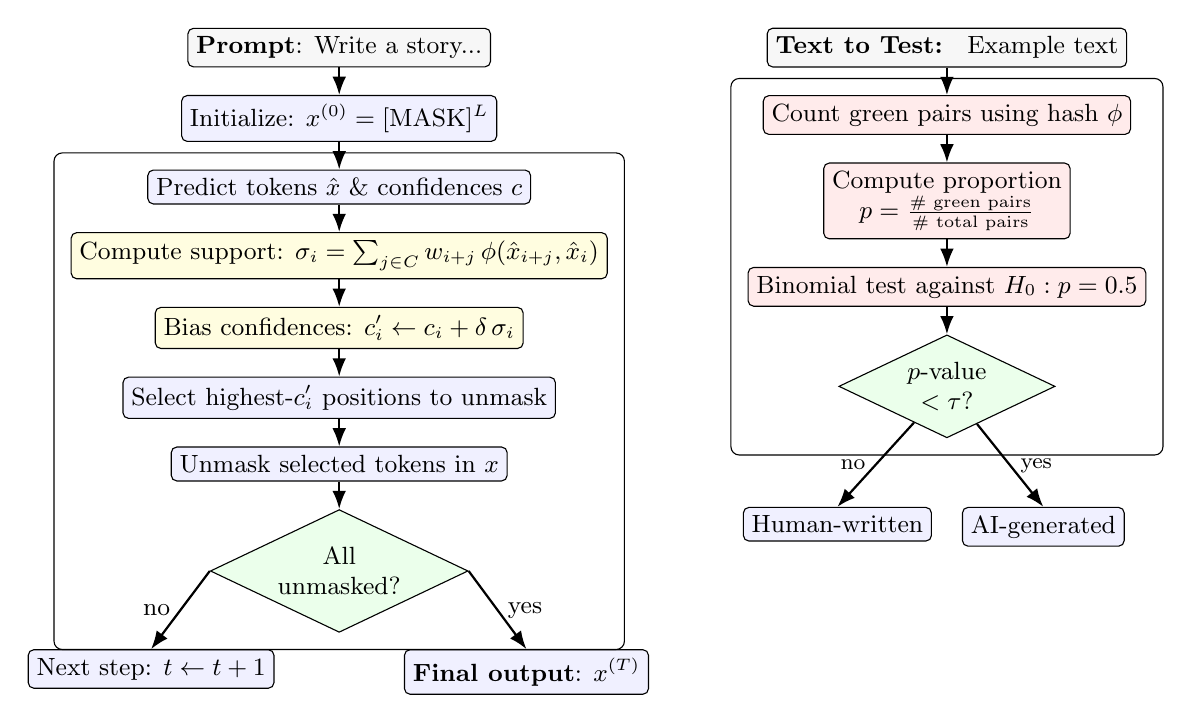
\begin{tikzpicture}[
  font=\small,
  node distance=3.5mm and 14mm,
  box/.style={draw, rounded corners=2pt, align=center, inner sep=3pt},
  proc/.style={box, fill=blue!6},
  data/.style={box, fill=gray!6},
  accent/.style={box, fill=yellow!12},
  decision/.style={shape=diamond, draw, align=center, inner sep=2pt, aspect=2.1, fill=green!8},
  detect/.style={box, fill=red!8},
  arrow/.style={-Latex, thick}
]
\node[data] (prompt) at (-2,0) {\textbf{Prompt}: Write a story...};
\node[proc, below=of prompt] (init) {Initialize: $x^{(0)}=[\text{MASK}]^L$};
\node[proc, below=of init] (predict) {Predict tokens $\hat{x}$ \& confidences $c$};
\node[accent, below=of predict] (score) {Compute support: $\sigma_i=\sum_{j\in C} w_{i+j}\,\phi(\hat{x}_{i+j},\hat{x}_i)$};
\node[accent, below=of score] (bias) {Bias confidences: $c'_i \leftarrow c_i + \delta\,\sigma_i$};
\node[proc, below=of bias] (select) {Select highest-$c'_i$ positions to unmask};
\node[proc, below=of select] (unmask) {Unmask selected tokens in $x$};
\node[decision, below=of unmask] (done) {All\\unmasked?};
\node[proc, below left=6mm and 0mm of done] (repeat) {Next step: $t\leftarrow t+1$};
\node[proc, below right=6mm and 0mm of done] (final) {\textbf{Final output}: $x^{(T)}$};
\node[fit=(predict)(score)(bias)(select)(unmask)(done),
      draw, rounded corners=3pt, inner sep=6pt] (iterbox) {};
\coordinate (loopleft) at ([xshift=-14mm]iterbox.west);
\draw[arrow] (prompt) -- (init);
\draw[arrow] (init) -- (predict);
\draw[arrow] (predict) -- (score);
\draw[arrow] (score) -- (bias);
\draw[arrow] (bias) -- (select);
\draw[arrow] (select) -- (unmask);
\draw[arrow] (unmask) -- (done);
\draw[arrow] (done.west) -- node[left] {no} (repeat.north);
\draw[arrow] (done.east) -- node[right] {yes} (final.north);
\node[data, right=35mm of prompt] (testtext) {\textbf{Text to Test: } \text{Example text}};
\node[detect, below=of testtext] (countpairs) {Count green pairs using hash $\phi$};
\node[detect, below=of countpairs] (proportion) {Compute proportion\\$p = \frac{\text{\# green pairs}}{\text{\# total pairs}}$};
\node[detect, below=of proportion] (binomial) {Binomial test against $H_0: p = 0.5$};
\node[decision, below=of binomial] (threshold) {$p\text{-value}$\\$< \tau$?};
\node[proc, below left=12mm and -5mm of threshold] (human) {Human-written};
\node[proc, below right=12mm and -5mm of threshold] (ai) {AI-generated};\draw[arrow] (testtext) -- (countpairs);
\draw[arrow] (countpairs) -- (proportion);
\draw[arrow] (proportion) -- (binomial);
\draw[arrow] (binomial) -- (threshold);
\draw[arrow] (threshold) -- node[left,font=\footnotesize] {no} (human.north);
\draw[arrow] (threshold) -- node[right,font=\footnotesize] {yes} (ai.north);
\node[fit=(countpairs)(proportion)(binomial)(threshold),
      draw, rounded corners=3pt, inner sep=6pt] (detectbox) {};
\end{tikzpicture}
    \caption{Our watermark (Left) Generation algorithm (Right) Detection algorithm}
    \label{fig:genalgoformal}
\end{figure}

\section{Evaluation}
We apply our watermark to LLaDA-8b, although the algorithm is applicable to other DLMs \cite{nie2025large}. We randomly select prompts from the ELI5 dataset for evaluation \cite{fan2019eli5}. We generate responses between 100 and 400 tokens, at temperature 0.5. At lengths under 200, detection reliability is worse, as we need sufficient sample size for the binomial test. We measure watermark strength with true positive rate at a 1\% false positive rate threshold (TPR @ 1).

\textbf{Watermark Reliability}
Figure 2 shows that at generation length 400, our algorithm achieves a 97\% TPR @ 1 over 1000 different prompts. At generation length 200, TPR @ 1 drops to 74\%, which is due to the necessity of a sufficient sample size. Figure 3 compares TPR @ 1 at increasing levels of the scaling parameter, $\delta$, with each value of $\delta$ being evaluated on 100 different prompts. We have chosen $\delta$ = 2.0 for our experiments, since it results in high detection rate without as much impact to text quality. 

\textbf{}

\begin{figure}[h]
    \centering
    \begin{subfigure}[b]{0.48\linewidth}
        \centering
        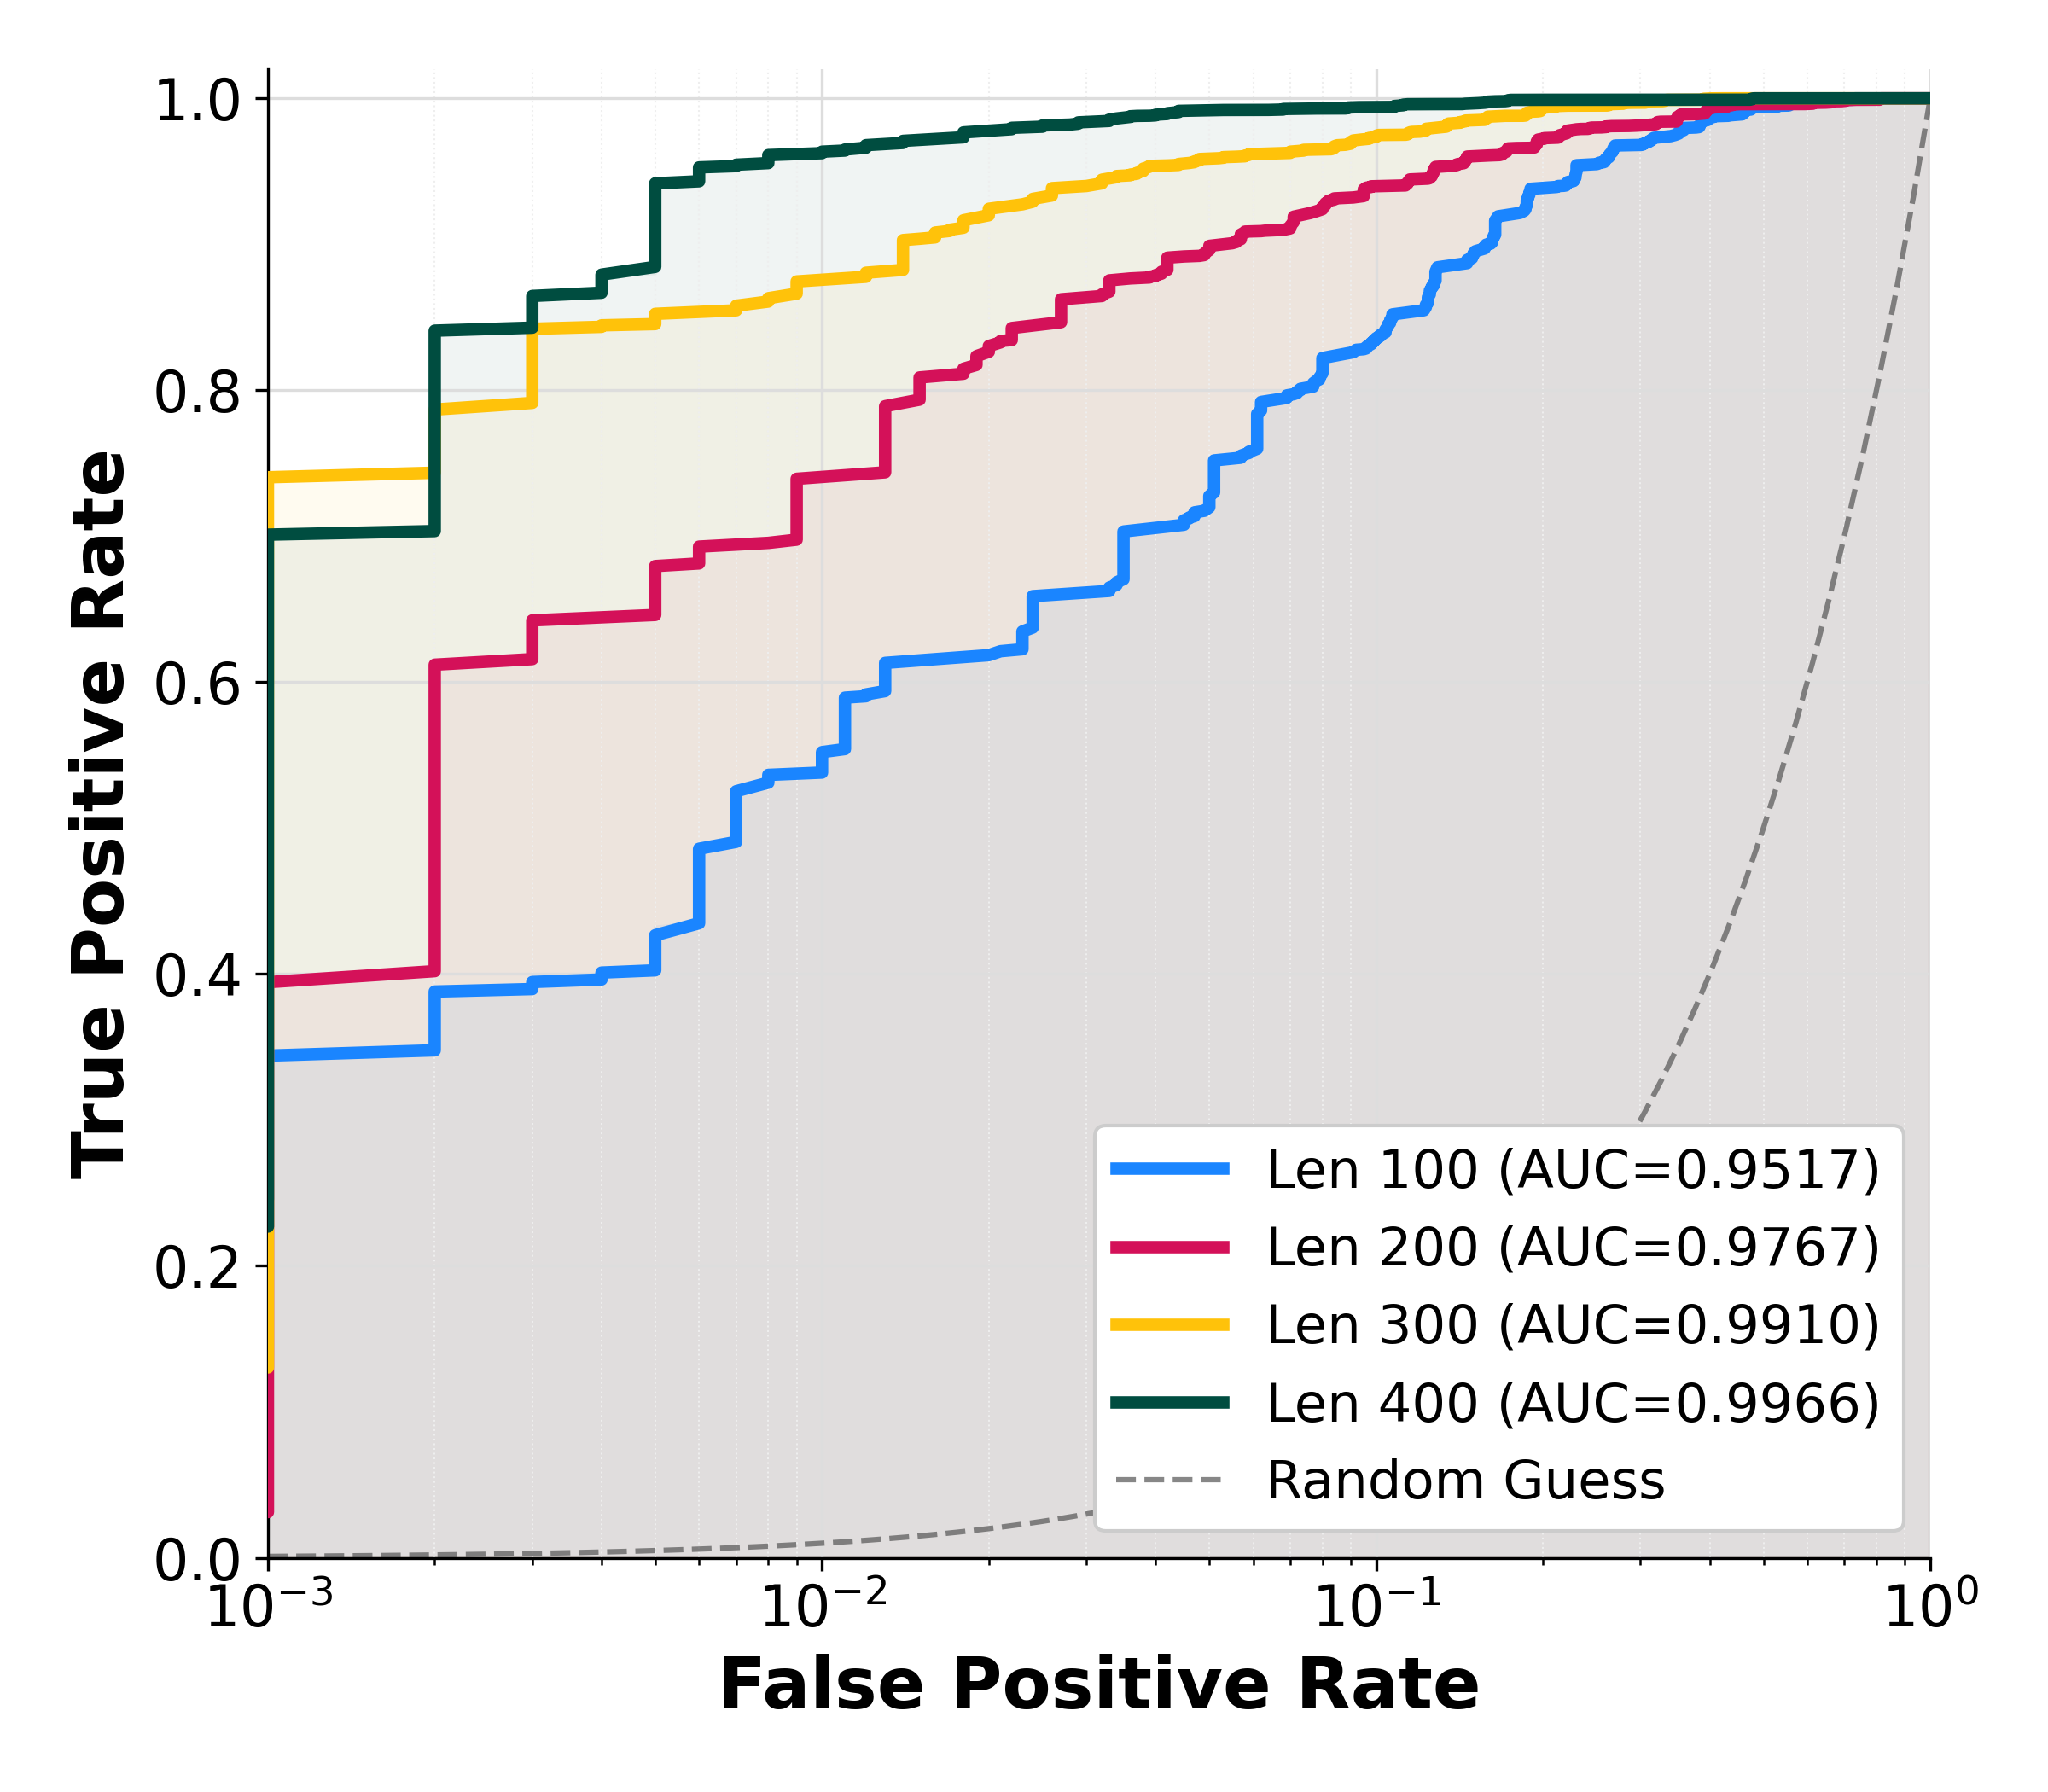
\includegraphics[width=\linewidth]{figures/roc_curve.png}
        \label{fig:roc_length}
    \end{subfigure}
    \hfill
    \begin{subfigure}[b]{0.48\linewidth}
        \centering
        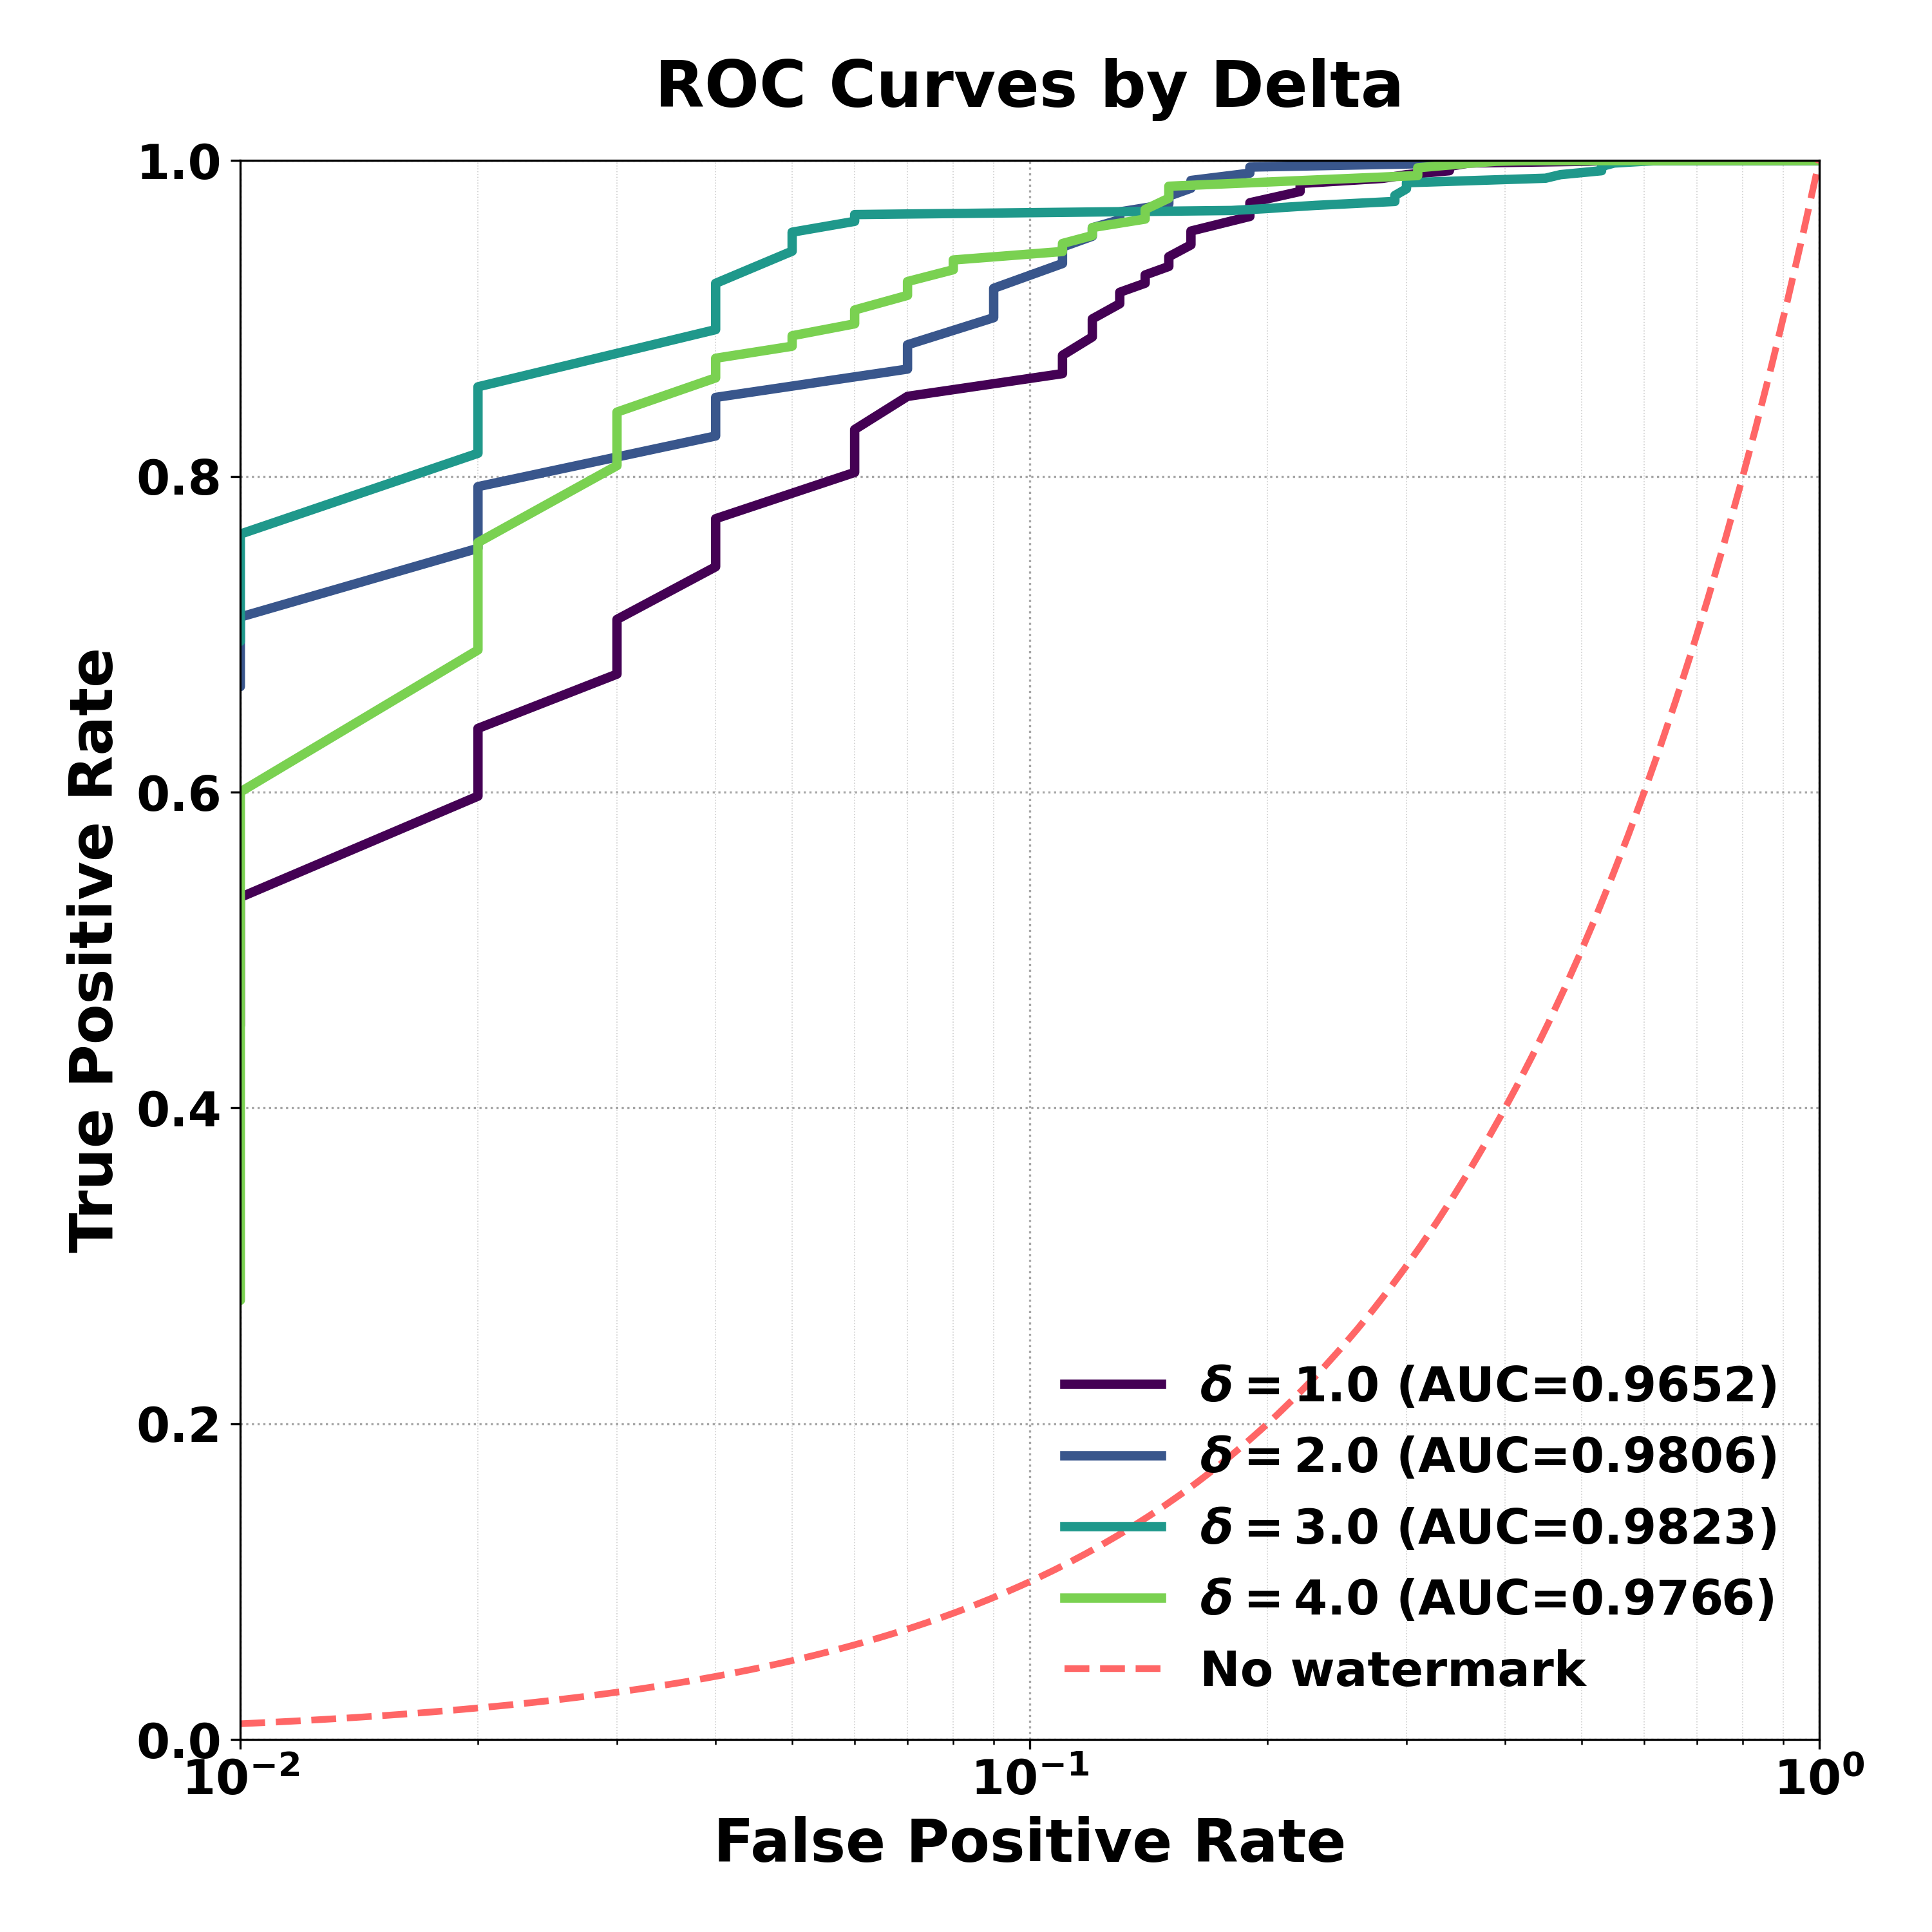
\includegraphics[width=\linewidth, trim=0 0 0 50, clip]{figures/roc.png}        
        \label{fig:roc_delta}
    \end{subfigure}
    \caption{Watermark Performance: ROC Curves Across Deltas and Token Lengths. TPR=FPR plotted in red. (Left) TPR plotted with FPR (1000 samples per length, fixed $\delta=2.0$). (Right) Varying deltas (fixed $N=400$).}
    \label{fig:roc_curve}
\end{figure}
\begin{figure}[h]
    \centering
    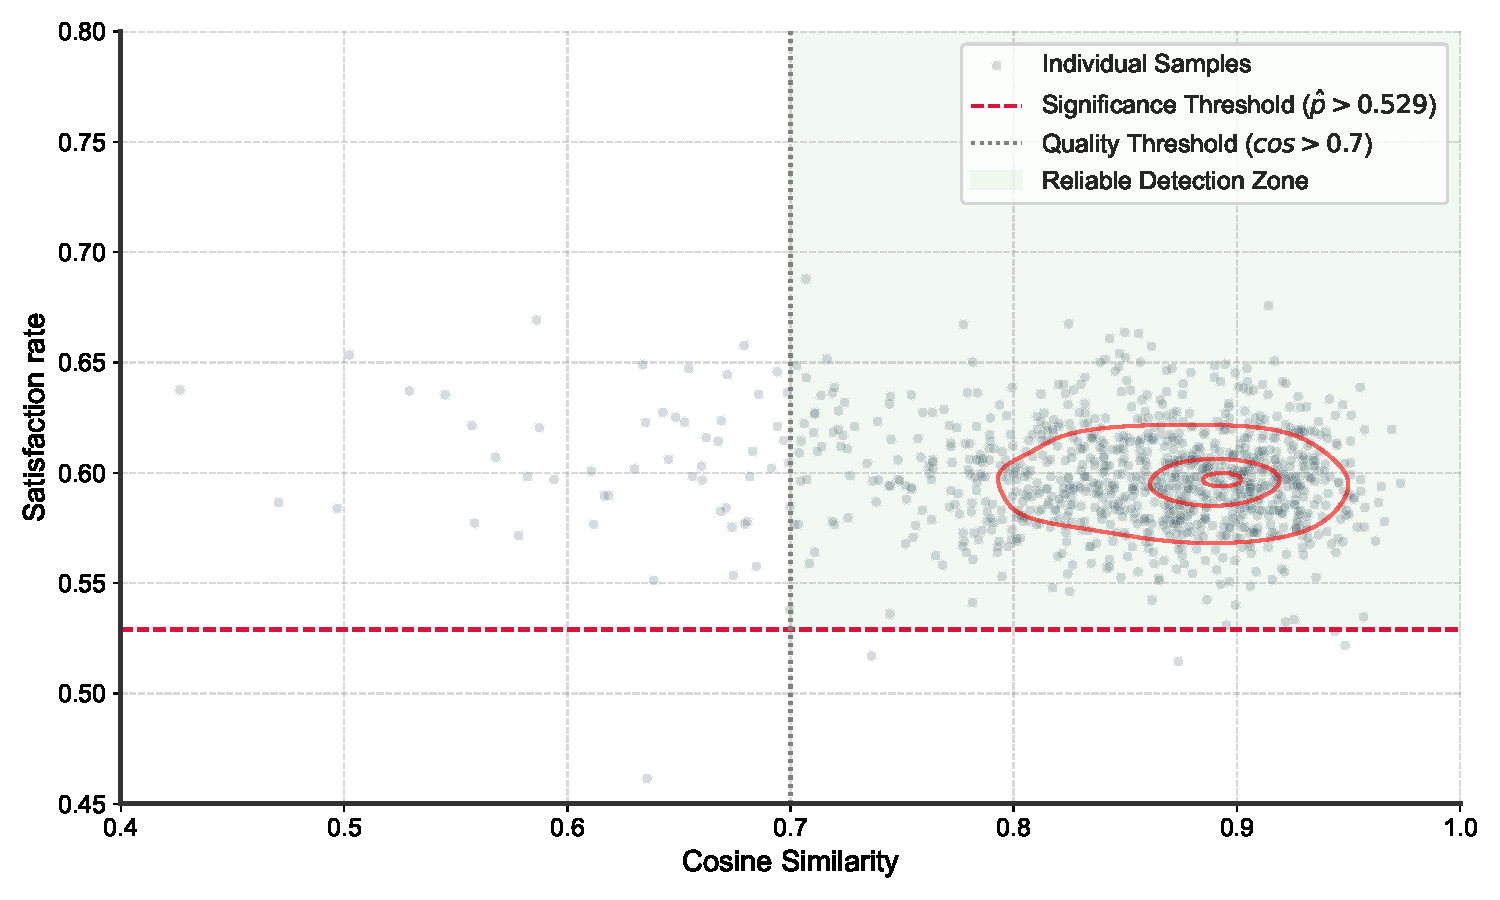
\includegraphics[width=0.8\linewidth]{figures/binomial_signal_analysis.pdf} 
    \caption{Signal Analysis (N=1000). Correlation between satisfaction rate and cosine similarity for outputs of length 400 ($\delta=2.0$). The concentration of samples is shown within the detection region (cos>0.7, $\hat{p}>0.529$), with contour rings at concentrations \{0.99, 0.9, 0.5\}.}
    \label{fig:signal_analysis}
\end{figure}


\clearpage


\bibliographystyle{plainnat}
\bibliography{references}
\section*{Additional Results}
\begin{figure}[h]
    \centering
    \begin{subfigure}{0.48\linewidth}
        \centering
        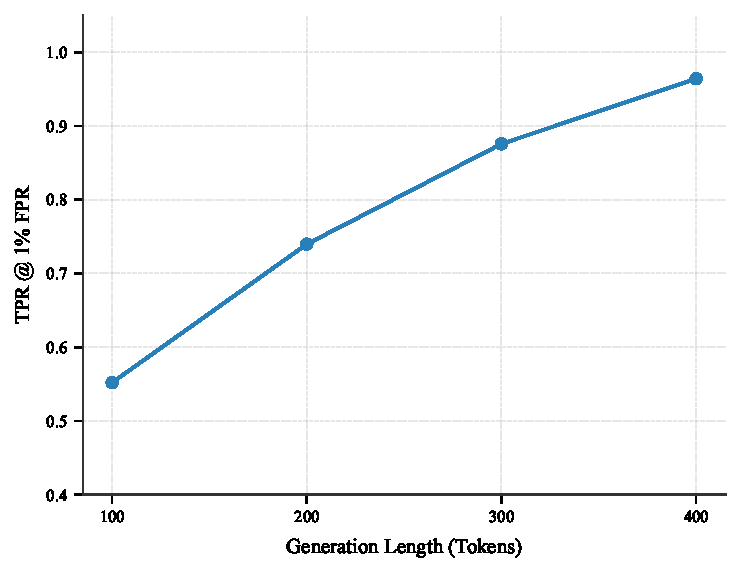
\includegraphics[width=\linewidth]{figures/length_performance_graph.pdf}
    \end{subfigure}
    \hfill
    \begin{subfigure}{0.48\linewidth}
        \centering
        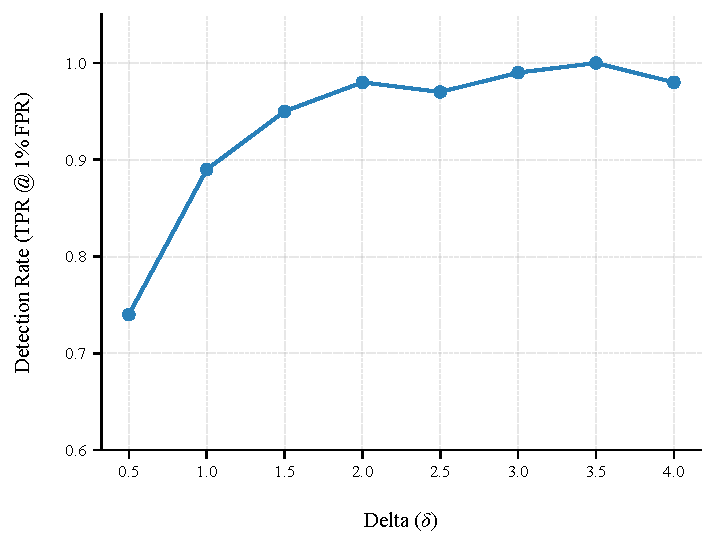
\includegraphics[width=\linewidth]{figures/line_graph.pdf}
    \end{subfigure}
    \caption{Detection Performance Analysis. Watermark reliability evaluated on the ELI5 dataset. (Left) TPR at 1\% FPR across varying generation lengths (1{,}000 samples per length, fixed $\delta=2.0$). (Right) Impact of scaling parameter $\delta$ on detection performance (100 samples per $\delta$, fixed generation length of 400 tokens).}
    \label{fig:accuracy}
\end{figure}
\section*{List of Theorems and Proofs}
\begin{theorem}[Selection-Step KL Divergence]
Let $P_{conf}$ be the original probability distribution over a candidate set, and $Q_{conf}$ be the watermarked distribution obtained by adding a bias vector $\mathbf{d}$ to the logits, where $0 \le d_i \le \delta k$. The Kullback-Leibler divergence is bounded by:
$$\mathrm{D}_{KL}(Q_{conf} \parallel P_{conf}) \le \delta k$$
\end{theorem}

\begin{proof}
Let the original logits for a vocabulary of size $V$ be $\mathbf{C} = (C_1, \dots, C_V)$, and the biased logits be $\mathbf{C'} = (C_1+d_1, \dots, C_V+d_V)$. The original and watermarked probability distributions, $P_{conf}$ and $Q_{conf}$, are obtained by applying the softmax function to these logits:
$$P_i = \frac{e^{C_i}}{Z_P}, \quad Q_i = \frac{e^{C_i+d_i}}{Z_Q}$$
where $Z_P = \sum_{j=1}^V e^{C_j}$ and $Z_Q = \sum_{j=1}^V e^{C_j+d_j}$ are the partition functions.

The Kullback-Leibler (KL) divergence from $Q_{conf}$ to $P_{conf}$ is defined as:
$$\mathrm{D}_{KL}(Q_{conf} \parallel P_{conf}) = \sum_{i=1}^V Q_i \log\frac{Q_i}{P_i}$$
The log-probability ratio for a single token $i$ is:
$$\log\frac{Q_i}{P_i} = \log\left(\frac{e^{C_i+d_i}/Z_Q}{e^{C_i}/Z_P}\right) = d_i - \log\frac{Z_Q}{Z_P}$$
Let $\Delta = \log(Z_Q/Z_P)$. The KL divergence can be written as:
$$\mathrm{D}_{KL}(Q_{conf} \parallel P_{conf}) = \sum_{i=1}^V Q_i (d_i - \Delta) = \left(\sum_{i=1}^V Q_i d_i\right) - \Delta$$
This is the expected bias minus the log-partition ratio. We can bound $\Delta$:
$$e^\Delta = \frac{Z_Q}{Z_P} = \frac{\sum_j e^{C_j+d_j}}{\sum_j e^{C_j}} = \sum_j \frac{e^{C_j}}{\sum_l e^{C_l}} e^{d_j} = \sum_j P_j e^{d_j} = \mathbb{E}_{j \sim P}[e^{d_j}]$$
Using the bounds on the bias, $0 \le d_j \le \delta k$, we have:
$$e^0 \le e^{d_j} \le e^{\delta k} \implies 1 \le e^{d_j} \le e^{\delta k}$$
The expectation is therefore bounded:
$$1 \le \mathbb{E}_{j \sim P}[e^{d_j}] \le e^{\delta k} \implies 0 \le \Delta \le \delta k$$
Thus, the KL divergence is bounded by the dynamic range of the log-likelihood ratio, $d_i - \Delta$. The maximum value of this term is bounded by $\max(d_i) - \min(\Delta) \le \delta k - 0 = \delta k$.
$$\mathrm{D}_{KL}(Q_{conf} \parallel P_{conf}) = \sum_i Q_i(d_i - \Delta) \le \sum_i Q_i(\delta k - 0) = \delta k$$
This completes the proof.
\end{proof}

\begin{theorem}[Perplexity Degradation]
Let $PPL_{orig}$ be the perplexity of the base model and $PPL_{wm}$ be the perplexity of the watermarked text evaluated by the base model. The degradation is bounded by:
$$PPL_{wm} \le PPL_{orig} \cdot e^{\delta k}$$
\end{theorem}

\begin{proof}
The perplexity of a text sequence $T=(t_1, \dots, t_N)$ evaluated by a model with probability distribution $P$ is defined as the exponential of the cross-entropy:
$$PPL_{wm} = \exp\left(H(T, P)\right) = \exp\left(-\frac{1}{N}\sum_{i=1}^N \log P(t_i|t_{<i})\right)$$
In our case, the watermarked text is generated from the distribution $Q$, so we are interested in the perplexity of text from $Q$ evaluated by $P$. This is the cross-entropy perplexity $PPL(Q,P)$. The perplexity of the original model on its own generated text is $PPL(P,P) = \exp(H(P))$, where $H(P)$ is the entropy of the distribution $P$.
The cross-entropy $H(Q,P)$ can be decomposed as:
$$H(Q,P) = H(Q) + \mathrm{D}_{KL}(Q \parallel P)$$
where $H(Q)$ is the entropy of the watermarked distribution.
From Theorem 1, we know that the KL divergence at each step is bounded:
$$\mathrm{D}_{KL}(Q(\cdot|t_{<i}) \parallel P(\cdot|t_{<i})) \le \delta k$$
Averaging over all generation steps, the full sequence KL divergence is also bounded by $\delta k$.
The application of a watermark bias generally reduces the entropy of the distribution, as it makes the model's choices more deterministic. Thus, we can assume that $H(Q) \le H(P)$.
Combining these results:
$$\log(PPL_{wm}) = H(Q,P) = H(Q) + \mathrm{D}_{KL}(Q \parallel P) \le H(P) + \delta k$$
Since $\log(PPL_{orig}) = H(P)$, we have:
$$\log(PPL_{wm}) \le \log(PPL_{orig}) + \delta k$$
Exponentiating both sides gives the final result:
$$PPL_{wm} \le PPL_{orig} \cdot e^{\delta k}$$
\end{proof}

\begin{theorem}[Expected Green Pair Rate Bounds]
Assuming a prior green probability $E[P_g] = p_0 = 0.5$, the expected watermark satisfaction rate $E[S_{wm}]$ is bounded as follows:
$$\frac{(e^\delta - 1)p_0(1 - p_0)}{1 + (e^\delta - 1)p_0} \le E[S_{wm}] - p_0 \le \frac{1}{1 + e^{-\delta}} - p_0$$
\end{theorem}

\begin{proof}
Let $P_g$ be the prior probability of a token being green, which is a random variable. We assume that without watermarking, the expected green probability is $E[P_g] = p_0 = 0.5$. The watermarking process adds a bias $\delta$ to the logits of green tokens. The probability of selecting a green token, given a prior probability $p$, becomes:
$$f(p) = \frac{p e^\delta}{p e^\delta + (1-p)}$$
The expected satisfaction rate of the watermark, $E[S_{wm}]$, is the expectation of this function over the distribution of $P_g$, i.e., $E[f(P_g)]$.

\textbf{Upper Bound:}
The function $f(p)$ is concave for $\delta > 0$. The second derivative with respect to $p$ is:
$$f''(p) = -\frac{2e^\delta(e^\delta-1)}{(p(e^\delta-1)+1)^3}$$
Since $\delta > 0$, $e^\delta > 1$, and the denominator is positive, $f''(p) < 0$.
By Jensen's inequality for concave functions, $E[f(X)] \le f(E[X])$. Applying this to our case:
$$E[S_{wm}] = E[f(P_g)] \le f(E[P_g]) = f(p_0)$$
Substituting $p_0=0.5$:
$$E[S_{wm}] \le \frac{0.5 e^\delta}{0.5 e^\delta + 0.5} = \frac{e^\delta}{e^\delta+1} = \frac{1}{1+e^{-\delta}}$$
The increase over the baseline $p_0$ is therefore:
$$E[S_{wm}] - p_0 \le \frac{1}{1+e^{-\delta}} - 0.5$$

\textbf{Lower Bound:}
The increase in the probability of selecting a green token for a given prior $p$ is:
$$f(p) - p = \frac{p(1-p)(e^\delta-1)}{1+p(e^\delta-1)}$$
The lower bound in the theorem is the expectation of this quantity, which is a known result for Bernoulli sampling. This serves as a lower bound for more sophisticated sampling methods like top-k or nucleus sampling, which are designed to increase the likelihood of selecting high-probability (and thus potentially green) tokens more than simple biased sampling. The greedy nature of these methods ensures a higher satisfaction rate than the probabilistic Bernoulli scheme, making this a valid lower bound.
\end{proof}

\begin{theorem}[False Positive (Forgery) Probability]
The probability that a non-watermarked text $T$ of length $N$ naturally achieves a satisfaction rate $S \ge S_{thresh}$ is bounded by:
$$P(S \ge S_{thresh}) \le \exp\left( -\frac{N}{2} (S_{thresh} - p_0)^2 \right)$$
\end{theorem}

\begin{proof}
Let $T = (t_1, \dots, t_N)$ be a non-watermarked text. Let $f(T)$ be the number of green pairs in the text. With a context window of size $k$, there are approximately $M \approx Nk$ pairs in the text. For a non-watermarked text, the probability of a pair being green is $p_0 = 0.5$. The expected number of green pairs is $E[f(T)] = M p_0$. The satisfaction rate is $S(T) = f(T)/M$.

We use McDiarmid's inequality to bound the probability of deviation from the mean. The inequality states that for a function $f$ with the bounded differences property,
$$P(f(T) - E[f(T)] \ge \epsilon) \le \exp\left( -\frac{2\epsilon^2}{\sum_{i=1}^N c_i^2} \right)$$
where $c_i$ is the maximum change in $f$ when the $i$-th input variable is changed. In our case, changing a single token $t_i$ can affect the color of at most $2k$ pairs (the pairs where $t_i$ is the left or right token). Therefore, the function $f(T)$ has a bounded difference with $c_i = 2k$.

The sum of squared differences is $\sum_{i=1}^N c_i^2 = N (2k)^2 = 4Nk^2$.
We are interested in the probability $P(S(T) \ge S_{thresh})$, which is equivalent to $P(f(T) \ge M S_{thresh})$.
Let $\epsilon = M S_{thresh} - E[f(T)] = M(S_{thresh} - p_0)$.
Plugging this into McDiarmid's inequality:
$$P(S(T) \ge S_{thresh}) \le \exp\left( -\frac{2(M(S_{thresh} - p_0))^2}{4Nk^2} \right)$$
Substituting $M \approx Nk$:
$$P(S(T) \ge S_{thresh}) \le \exp\left( -\frac{2(Nk(S_{thresh} - p_0))^2}{4Nk^2} \right) = \exp\left( -\frac{2N^2k^2(S_{thresh} - p_0)^2}{4Nk^2} \right)$$
$$P(S(T) \ge S_{thresh}) \le \exp\left( -\frac{N}{2}(S_{thresh} - p_0)^2 \right)$$
This gives the bound for the false positive probability.
\end{proof}

\begin{theorem}[False Negative Probability]
The probability that a watermarked text fails to exceed the threshold $S_{thresh}$ is bounded by:
$$P(S_{wm} < S_{thresh}) \le \exp\left( -\frac{N}{2} (E[S_{wm}] - S_{thresh})^2 \right)$$
\end{theorem}

\begin{proof}
Let $T_{wm}$ be a watermarked text of length $N$. Let $f(T_{wm})$ be the number of green pairs. The satisfaction rate is $S_{wm}(T_{wm}) = f(T_{wm})/M$, where $M \approx Nk$ is the total number of pairs. The expected satisfaction rate is $E[S_{wm}]$, and the expected number of green pairs is $E[f(T_{wm})] = M \cdot E[S_{wm}]$.

A false negative occurs if the satisfaction rate of the watermarked text is below the detection threshold, i.e., $S_{wm} < S_{thresh}$. This is equivalent to $f(T_{wm}) < M S_{thresh}$.
We can express this as a deviation from the mean:
$$E[f(T_{wm})] - f(T_{wm}) > E[f(T_{wm})] - M S_{thresh} = M(E[S_{wm}] - S_{thresh})$$
Let $\epsilon = M(E[S_{wm}] - S_{thresh})$. We use McDiarmid's inequality for the lower tail:
$$P(E[f(T)] - f(T) \ge \epsilon) \le \exp\left( -\frac{2\epsilon^2}{\sum_{i=1}^N c_i^2} \right)$$
As in the false positive case, the function $f$ has the bounded difference property with $c_i=2k$, so $\sum c_i^2 = 4Nk^2$.
Substituting $\epsilon$ into the inequality:
$$P(S_{wm} < S_{thresh}) \le \exp\left( -\frac{2(M(E[S_{wm}] - S_{thresh}))^2}{4Nk^2} \right)$$
Using the approximation $M \approx Nk$:
$$P(S_{wm} < S_{thresh}) \le \exp\left( -\frac{2(Nk(E[S_{wm}] - S_{thresh}))^2}{4Nk^2} \right) = \exp\left( -\frac{2N^2k^2(E[S_{wm}] - S_{thresh})^2}{4Nk^2} \right)$$
$$P(S_{wm} < S_{thresh}) \le \exp\left( -\frac{N}{2}(E[S_{wm}] - S_{thresh})^2 \right)$$
This provides the bound for the false negative probability.
\end{proof}

\begin{theorem}[Robustness to Edits]
The minimum edit distance $E$ required to degrade the watermark satisfaction from $S_{wm}$ to a threshold $S_{thresh}$ is lower-bounded by:
$$E \ge \frac{N}{2} (S_{wm} - S_{thresh})$$
\end{theorem}

\begin{proof}
Let $T$ be a watermarked text of length $N$ with a satisfaction rate $S_{wm}$. The number of green pairs is $f(T) = M S_{wm}$, where $M \approx Nk$ is the total number of pairs.
To remove the watermark, an attacker must edit the text to produce a new text $T'$ with a satisfaction rate $S'_{wm} < S_{thresh}$.
The number of green pairs that must be flipped from green to not-green is:
$$\Delta_{pairs} = f(T) - f(T') > M(S_{wm} - S_{thresh})$$
A single edit to the text (substitution, insertion, or deletion) at position $i$ can affect the color of pairs that include the token $t_i$. With a context window of size $k$, a token can be part of at most $2k$ pairs (as the left or right token in a pair).
In the most effective attack, a single edit flips the color of the maximum possible number of green pairs. This maximum is $2k$.
Let $E$ be the number of edits. The total number of pairs whose color can be changed is at most $E \cdot 2k$.
To achieve the goal of reducing the satisfaction rate below the threshold, the number of edits must satisfy:
$$E \cdot 2k \ge \Delta_{pairs} > M(S_{wm} - S_{thresh})$$
Using the approximation $M \approx Nk$:
$$E \cdot 2k > Nk(S_{wm} - S_{thresh})$$
$$E > \frac{Nk}{2k}(S_{wm} - S_{thresh}) = \frac{N}{2}(S_{wm} - S_{thresh})$$
Since the number of edits $E$ must be an integer, the lower bound is:
$$E \ge \left\lfloor \frac{N}{2}(S_{wm} - S_{thresh}) \right\rfloor + 1$$
The theorem provides a slightly looser but more standard form of this bound.
\end{proof}

\end{document}